\section{概述}

\subsection{查询处理的基本步骤}

1.解析与转换

2.优化

3.评估

\begin{figure}[H]
    \centering
    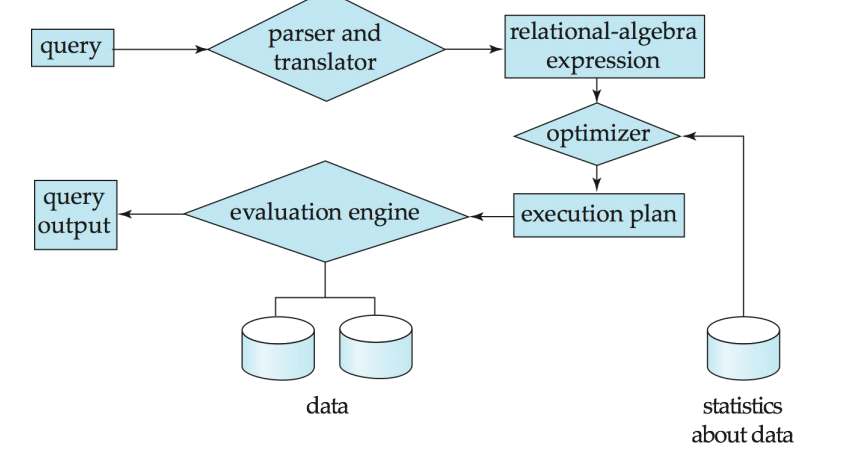
\includegraphics[width=0.8\linewidth]{image1.png}
    \caption{基本步骤}
    \label{}
\end{figure}

解析与翻译(语法分析与翻译)与编译器对比:解析器检查语法,验证关系;将查询转换为其内部形式---扩展关系代数(ERA)。

\noindent评估:查询执行引擎获取查询评估计划,执行该计划,并返回查询的答案。

评估计划精确地定义了每个操作使用的算法,以及操作的执行如何协调。

\noindent优化---为什么?

对于给定的SQL查询,可能有许多等价的关系代数表达式。

例如:\texttt{select balance from account where balance > 2500}.
$$\sigma_{balance>2500}(\prod_{balance}(account))$$
$$\prod_{balance}(\sigma_{balance>2500}(account))$$

每个关系代数运算都可以使用几种不同的算法之一进行评估。

相应地,一个关系代数表达式可以通过多种方式进行评估。

指定详细评估策略的带注释表达式称为评估计划。

\subsection{基本步骤:优化}

(1)找出各种等价的关系代数表达式。

(2)一组指定详细评估策略的基本操作序列称为查询执行计划或查询评估计划。

(3)查询优化:在所有等效的评估计划中,选择成本最低的那个。成本考虑两个因素:成本取决于执行算法,还可以使用数据库目录中的统计信息来估算成本。